\chapter{Introduction and State of the Art}
\label{c-intro}

\section{Neuroscience, neurons and their dynamics}
% \textit{What are neurons, its dynamics and what are the To-Dos}
Neuroscience is a wide and challenging field in science. It faces crucial questions, such as the neural mechanisms in the brain activity, how can those mechanisms outcome as human cognition or behavior, how is the information processed and transferred through neural activity, how are neural diseases generated and how can we detect and treat them. 
These questions and many more have been open problems that have intrigued scientific community since the first steps on the field. Neuroscience was born as a discipline from physiology, biochemistry and anatomy. As a broad field, it is approached from distinct perspectives and it is usually referred to by its subfields, e.g. Neurobiology, Neurophotonics, Neuropharmacology, Clinical Neuroscience, Developmental Neuroscience, Systems Neuroscience, Cognitive Neuroscience, Computational Neuroscience. All these fields aim to explain the brain performance either as a whole or in parts. They use different techniques and approaches where some of which give rise to entirely new fields, like Neuroimaging.

We cannot think or discuss about neuroscience without highlighting the work by Santiago Ramón y Cajal, crucial in the firsts steps on the understanding of brain dynamics \parencite{de_carlos_historical_2007,de_castro_editorial_2016,delgado-garcia_cajal_2015,de_castro_cajal_2019}. The idea of the "neuron doctrine" was a boost on the study of the brain, explaining and describing the structure of individual cells called \textit{neurons} that are able to connect and thus communicate by \textit{synapses}. In Figure \ref{cajal-neuron} there is one of his famous drawings of the description of a neuron.

\begin{figure}[htb!]
    \centering
    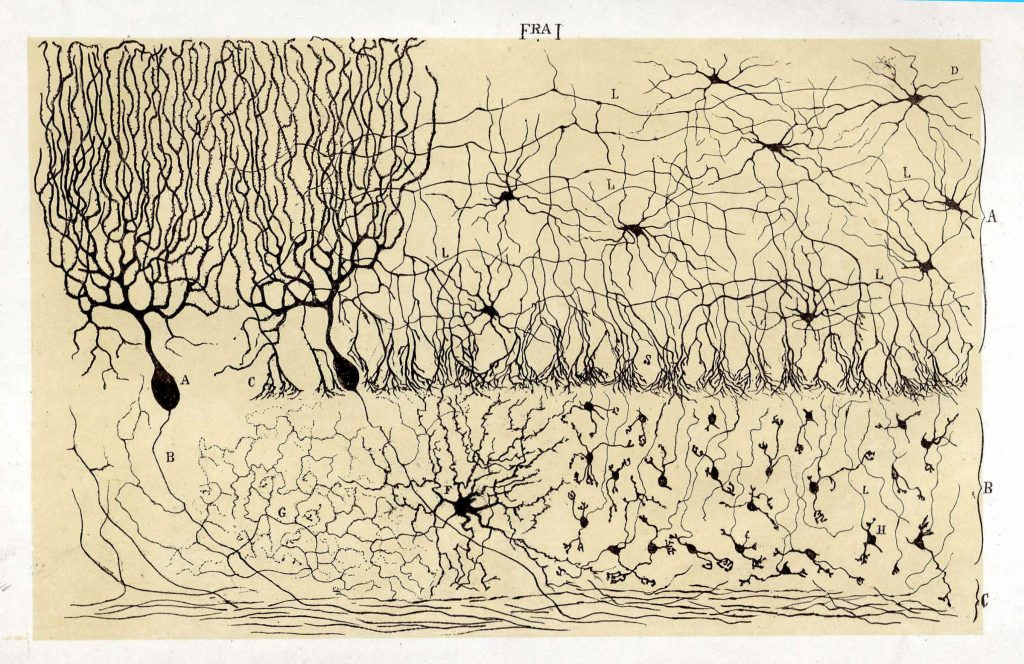
\includegraphics[width=\textwidth]{img/intro/CajalCerebellum.jpeg}
    % https://es.wikipedia.org/wiki/Doctrina_de_la_neurona#/media/Archivo:CajalCerebellum.jpg
    % https://microbioblog.es/la-fascinante-historia-de-la-reazione-nera
    \caption{Representation of Cerebellum neurons by Ramon y Cajal}
    \label{cajal-neuron}
\end{figure}

%From that starting point there have been important findings in the neurons types and structures, such as Glia cells \ref{}. 

As we have seen brain is a complex system and we can study it from many different prisms. In this thesis we follow a bottom-up approach. So we will analyze experimentally and theoretically the neural activity at ionic channels and small circuits (few synapses). Moreover, we will follow a Neurocomputational perspective, that will be defined in detail in subsection \ref{sec:computational neuroscience}. In the following lines we will approach the basis of neural activation from a computational perspective necessary for the reading flow of this document. We will focus not in their molecular properties but in the change of voltage that they are able to produce and how that inter-operates. 

\subsection{Neural activation}
Neurons are cells composed by axons (the information transfer tube), dendrites (the information reception point) and synapses (the process of information transfer). Also, as many other cells, it has a soma and although the generation of activity is a complex distributed event, to a great extent it is in the soma where the activity is processed. 

% As said there are many different ways to study neural dynamics, but a common descriptor for neural activity are action potentials. Action potentials are the 
Neural activity is often described by the potential alteration in the membrane caused by the flow of ionic channels and the conduction of nerve impulses by the axon. These variations of potential are called action potentials or spikes. We can see them as the minimal pieces of information in the process of its reception, modification and transmission carried out by the neurons. A more concrete definition of spike could be "an abrupt and transient change of membrane voltage that propagates to other neurons via a long protrusion called an axon" \parencite{izhikevich_dynamical_2007}. Thus when no activity is transferred through the axon, the potential is called resting potential, when this potential is altered by a voltage increase it is known as depolarization. After reaching a peak of voltage, the potential starts decreasing again. When the potential is more negative than the resting potential is known as hyperpolarization. In Figure \ref{fig:action potential} the action potential phases are depicted. 

\begin{figure}[htb!]
    \centering
    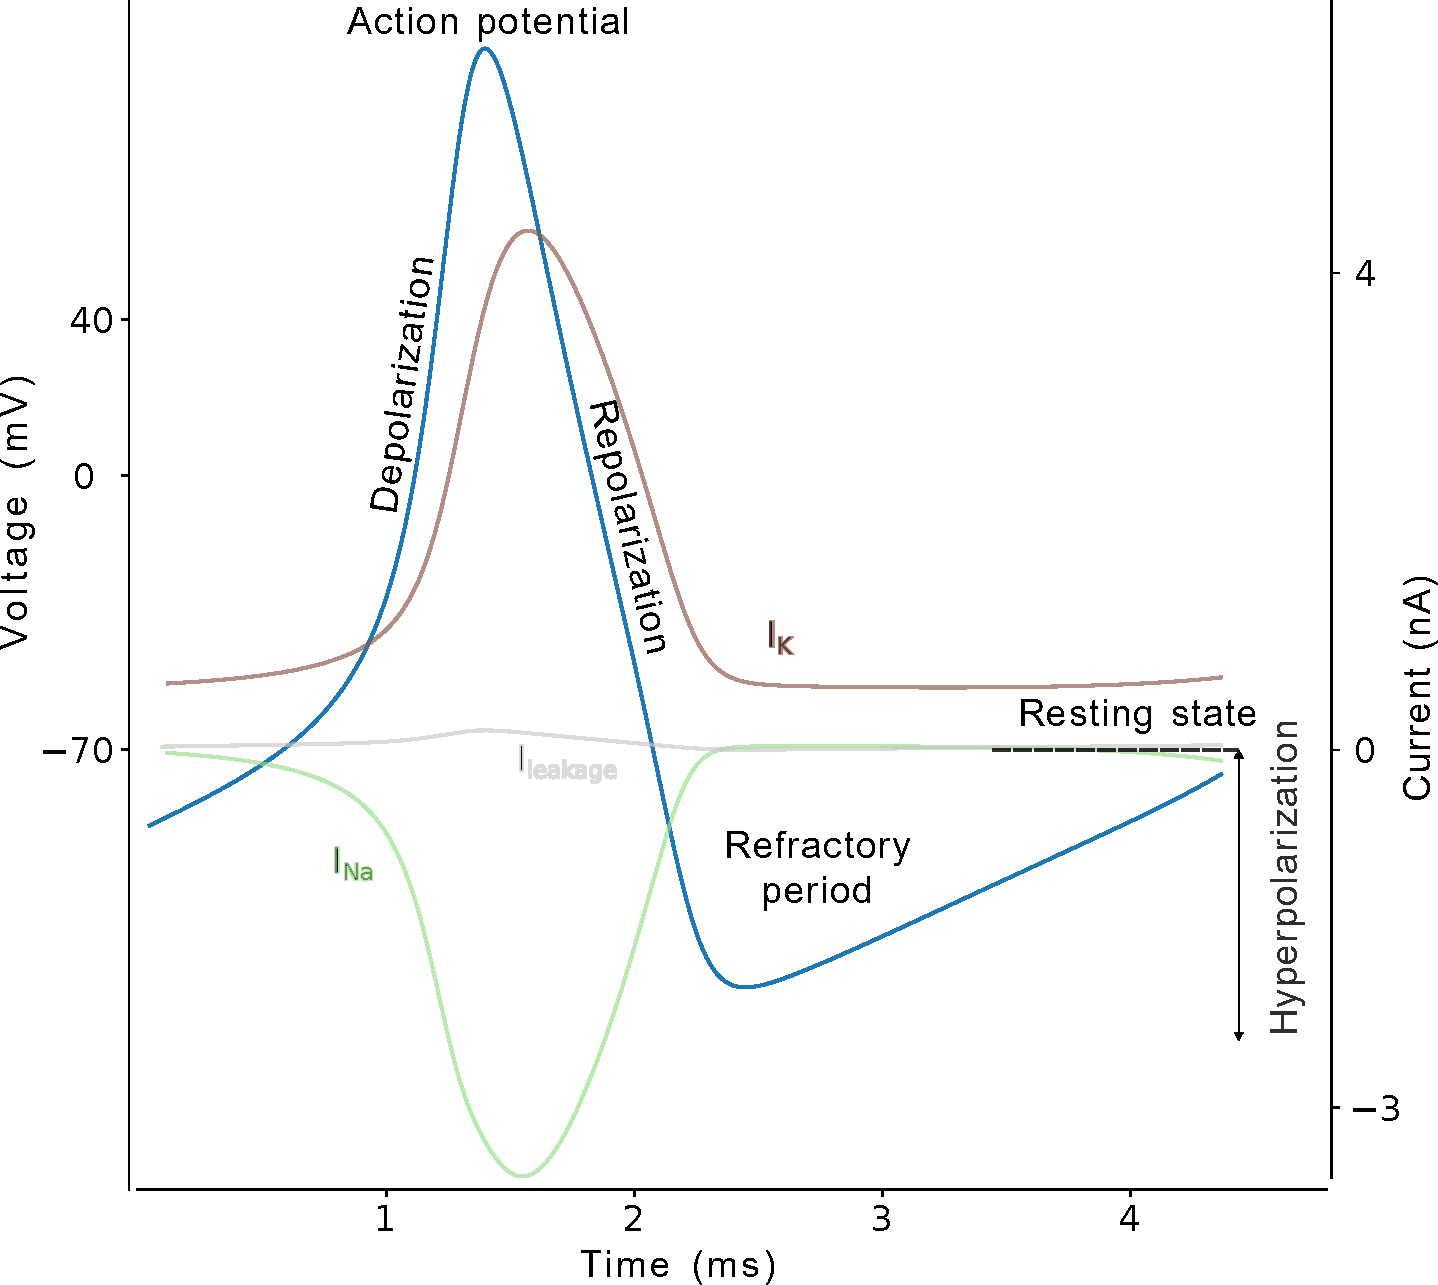
\includegraphics[width=0.8\textwidth]{img/intro/action_potential.pdf}
    \caption{Representation of phases and terminology of an action potential. (Adapted from Chris73, Wikimedia Commons, \href{https://creativecommons.org/licenses/by-sa/3.0/}{CC BY-SA 3.0}). }
    \label{fig:action potential}
\end{figure}

The neural activity is generated by the flow of different ionic channels that counterbalance the voltage value generating the action potential. The membrane can be composed by different ionic channels, and its dynamics are conditioned by that combination and the possible synaptic connections. These changes in dynamics can be manifested in different ways, but the most notorious ones are the shape of the action potential and the type of activity that they show. %p61 The Neuron 
For example, in Figure \ref{fig:spike-types} there is an example of two distinct action potentials with visible differences in their shape, of them presents a symmetrical shape, where depolarization and repolarization slopes are similar, whereas in the right waveform, there is a notable shoulder in the repolarization and its timescale is almost the double of example in (a).

\begin{figure}[htb!]
    \centering
    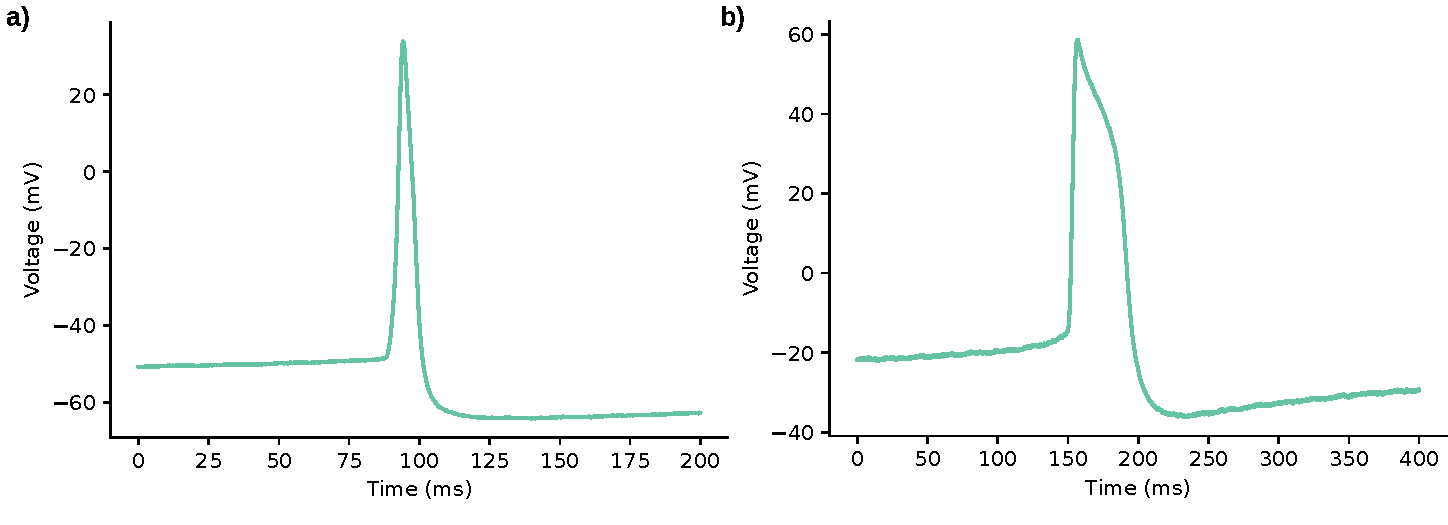
\includegraphics[width=\linewidth]{img/intro/spike-types.pdf}
    \caption{Examples of different spike shapes. Representation of two recordings from two different cells in \textit{Lymnaea stagnalis}. Left: symmetrical spike; right: shoulder shaped spike.}
    \label{fig:spike-types}
\end{figure}

If spikes are considered minimal pieces of information when coding the neural activity, the combination of these minimal information leads to new forms of information, also known as bursts. Although there is not a fixed description of a burst, and depending on the animal and system a burst might look different \parencite{russell_bursting_1978,palmu_detection_2010,lundqvist_gamma_2016}, there are some common features in bursts: combination of spikes (more than two), higher frequency, sustained depolarization, a hyperpolarization followed by a resting period called inter-burst interval (IBI). In Figure \ref{fig:spike_activity-types} there is an example of distinct neural activities from intracellular recordings, depending on the neuron, its composition and the circuit it is inmerse in, they present tonic firing (first column), at different rates, and bursting activity (second column). 
\begin{figure}[htb!]
    \centering
    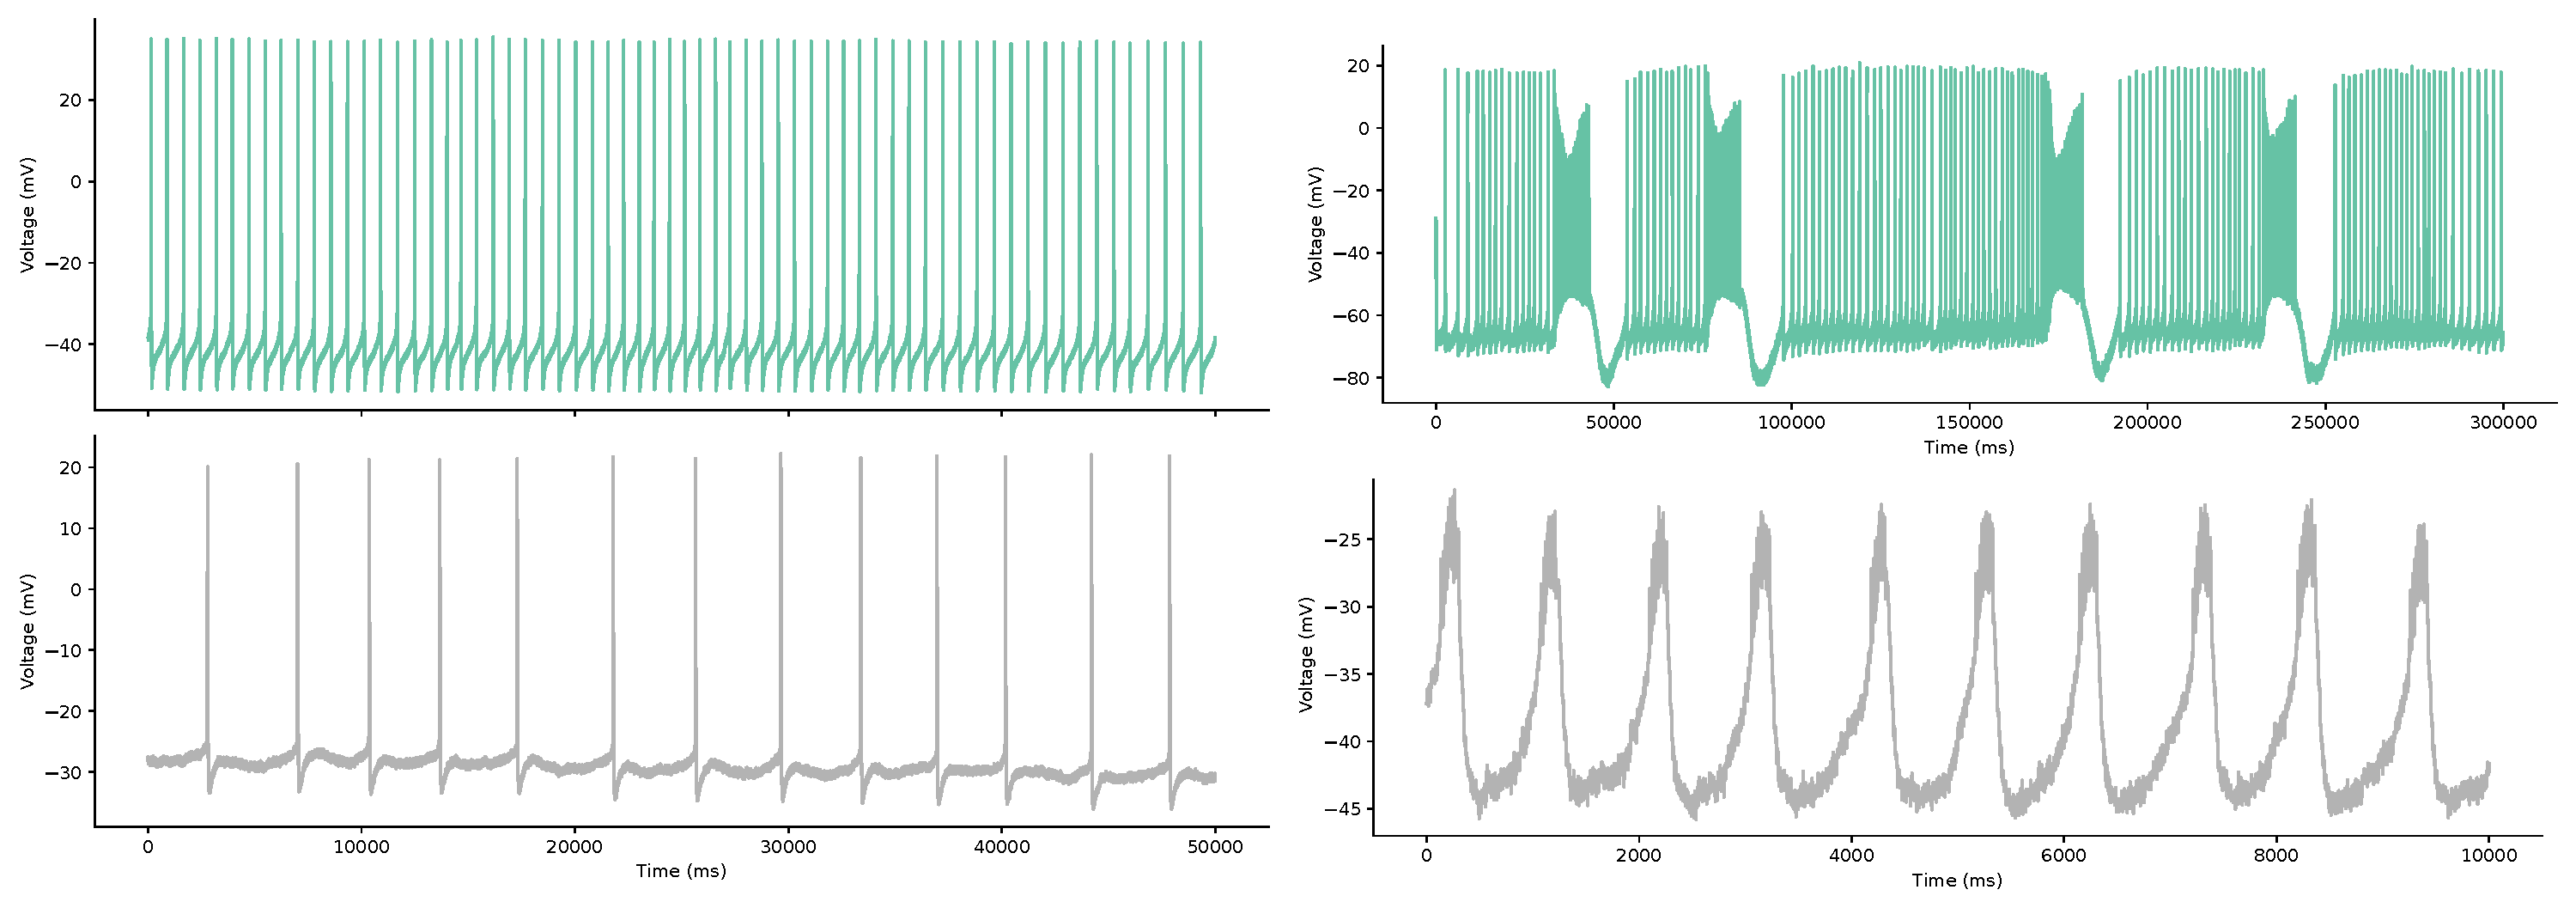
\includegraphics[width=\linewidth]{img/intro/spike_activity-types.pdf}
    \caption{Representation of two examples of different spiking activity. Left: two simultaneous intracellular recordings in \textit{Lymnaea stagnalis} showing tonic firing at two different frequencies. Right: Two examples of bursting activity, up from \textit{Lymnaea stagnalis} and bottom from \textit{Carcinus maenas}}
    \label{fig:spike_activity-types}
\end{figure}
Traditionally, neural code has been studied as information by the binarization of the activity i.e. an spike does or does not occur. Burst can also be part of this codification, either as a whole piece of information or as a complex box of data itself: "bursts are a family of firing patterns that trigger physiological mechanisms not engaged by the same number of spikes in relative isolation" \parencite{friedenberger_silences_2023}. Bursts can be originated either by internal activation, mostly by calcium channels or by the synaptic dynamics involving the corresponding cell (inhibition/excitation) (for an extended review see \parencite{friedenberger_silences_2023}). This is the case in Central Pattern Generators (CPGs) \parencite{Katz,steuer_central_2018} that will be discussed in detail bellow and in Chapter \ref{c-invariants-model}.

\subsection{Network dynamics}

Although analyzing the activity of a single neuron is important in terms of its dynamic, channels and the information it might carry, when talking about information processing and behavior, it is crucial to study the dynamics in circuits. Specially when talking about human brain and millions of neurons we divide the activity in groups and networks, exploring them as a whole. 
A circuit of neurons is defined by neurons interconnected by synapses.
We can find two big types of synapses, electrical or chemical. In Figure \ref{fig:synapse-types} there is a representation of both kinds. The main difference between them relay on how does the communication take place. Chemical synapses occur through the mediation of \textit{neurotransmitors}, where a presynaptic neuron liberates these molecules that are received and produce an alteration in a postsynaptic neuron. This is a fast mechanism that is conducted in the media. Thus, this connection is asymmetrical and unidirectional, whereas in electrical synapses we find a symmetrical and bidirectional connection. In those synapses, the neurons are almost attached by an structure called \textit{gap junction}, which "pipes" both neurons, in a tissued structure that constrains the leakage to the extracellular space. This communication is then faster than the chemical synapses, which in comparison has no delay. Activity in electrical connections is usually synchronous \parencite{levitan_neuron_2002}.

\begin{figure}[hbt!]
    \centering
    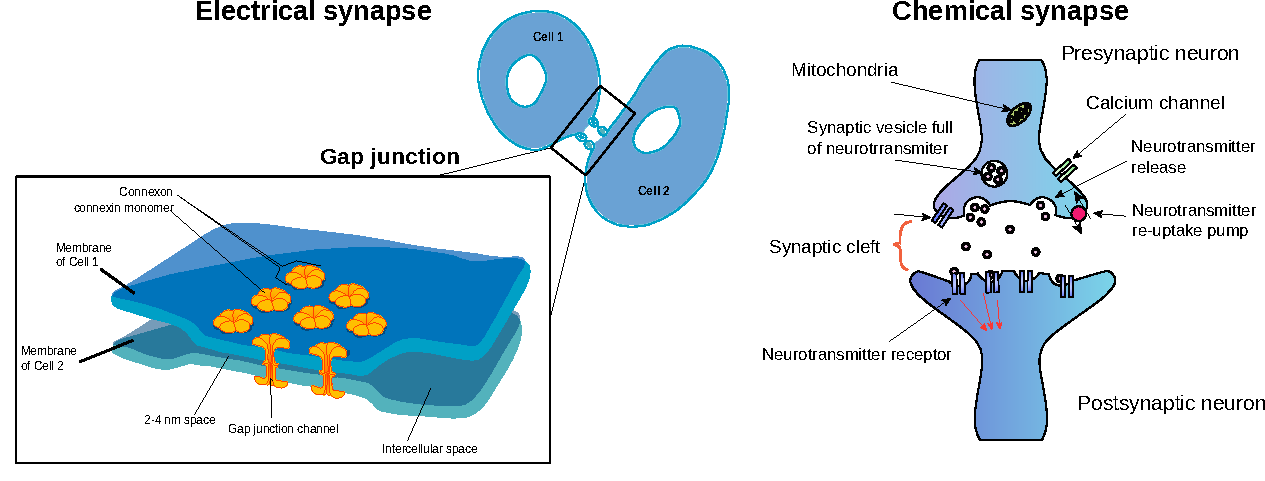
\includegraphics[width=\linewidth]{img/intro/synapses.pdf}
    \caption{Representation of synapses types. Left. Example of electrical synapse between two cells and diagram of gap junction (Adapted from \href{https://commons.wikimedia.org/wiki/File:Gap_cell_junction-en.svg}{Wikimedia Commons}). Right. Example of chemical synapse structure (Adapted from \href{https://commons.wikimedia.org/wiki/File:Synapse_diag1.svg}{Wikimedia Commons})}
    \label{fig:synapse-types}
\end{figure}

In circuits neurons can be connected by one or both types of synapses, and they usually are conected to other circuits or modulatory neurons. In Figure \ref{fig:neural circuits} there is an example of circuits at a cellular and macroscopic level.\todo{completar}

\begin{figure}[hbt!]
    \centering
    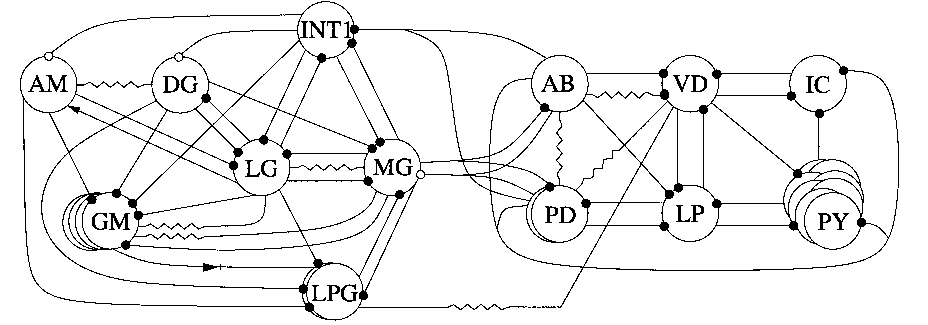
\includegraphics[width=0.64\textwidth]{img/intro/cpg diagram.png}
    \includegraphics[width=0.35\textwidth]{img/intro/The_Human_Connectome.png}
    \caption{Left. gastric and pyloric circuit scheme of \textit{Carcinus Maenas} \parencite{huerta_topology_2001}. Right. Conectome in human brain rendered from 20 subjects (By Andreashorn - Own work,\href{https://commons.wikimedia.org/w/index.php?curid=41581320}{CC BY-SA 4.0})}
    \label{fig:neural circuits}
\end{figure}

\section{The sequential nature of neural dynamics}
%the complex landscape of unanswered questions in the field of neuroscience, from a bottom-up approach.
Brain dynamics can be described as a sequence of interactions, from molecules to motor movement, a hierarchy of temporal scales \parencite{kiebel_hierarchy_2008}. This sequential nature of behavior and signal processing occurs at different time scales (from ionic channels activation to sensory input processing). Its study reveal fundamental aspects of brain function and cognition, e.g., impulse transmission, executive function, spatial processing or memory.

% There are many important cognitive processes that rely in sequential processes such as perception, memory, decision making, attention and emotion. %Binding \parencite{Michel and coegin 2018, Ravinovich 2020, He 2018}.
% Sequentiallity involves complex pieces of dynamical activity, that when incapsulated as units, can be seen as a chain of events with sequential behaviour \parencite{Ravinovich,2023}.


% Sequential activvation for unsuppervised learning/activity.

%Principles of Brain Dynamics: Global State Interaction Book
%https://www.frontiersin.org/articles/10.3389/fnsys.2014.00219/full
%https://www.ncbi.nlm.nih.gov/pmc/articles/PMC8367843/


%Kiebel 2009
%"Dynamic sequences are generated on various time-scales"
%"Brain is a recognition system that uses an internal model of its environment"

%Kiebel 2008
%"Many aspects of brain function can be understood in terms of a hierarchy of temporal scales at which representations of the environment evolve"


Temporal processing can be defined as the decoding of a generated temporal code. A common example of temporal processing is usually speech, where sequential patterns are present in the structure of phrases, as a sequences of syllables and silences \parencite{kiebel_recognizing_2009}. In this line, an extended case of study is the birdsong, which has this similarity to human's speech, as they process sequences of syllables \parencite{prather_brains_2017,fishbein_sound_2019}. Beyond speech, sequential processing is also present in the motor movement, from muscle activation to repetitive coordinated actions such as rhythmic tapping or music performance \parencite{ding_temporal_2017}. Also, there are many important cognitive processes that rely in sequential mechanisms such as perception, memory, decision making, attention and emotion \parencite{michel_eeg_2018, he_robust_2018, rabinovich_sequential_2020}.

However, it is not clear how exactly the brain processes time. In contrast to the theory of a central clock that manages time for every behavioral task, it is extended the theory of a distributed time processing \parencite{buonomano_temporal_1995,ivry_representation_1996}. For that to be processed, but maintaining effective responses, especially in movement, there is a need of circuits that manage the sequential rhythmic activity. This is the case of Central Pattern Generators (CPGs), closed circuits of neurons that activate sequentially in mutual inhibition and generate coordinated motor activity. They are present in many systems, from insects to humans \parencite{pearson_central_1972,marder_central_2001,mackay-lyons_central_2002,minassian_human_2017}. There are a few key aspects that makes this circuit an interesting case of study. First, the neurons in the closed-topology are able to maintain a rhythmic activity in an autonomous manner by mutual inhibition. Second, the activity is flexible enough to adapt to changes in the context, e.g., variations in the terrain while walking. Finally, it is present in many systems and in some of them there is a direct transcription between the neurons in the circuit and the motor movement they produce. For example, in the stomatogastric CPG in the crab \textit{C. maenas}, in charge of the pylorus movement, the PD (pyloric dilator), LP (Lateral Pyloric) and PY (PYloric) neurons correspond to the pylorus dilatation, pylorus close and contraction of the rostral constrictor to move food particles \parencite{selverston_oscillations_2006}.

\begin{figure}[hbt!]
	\centering
	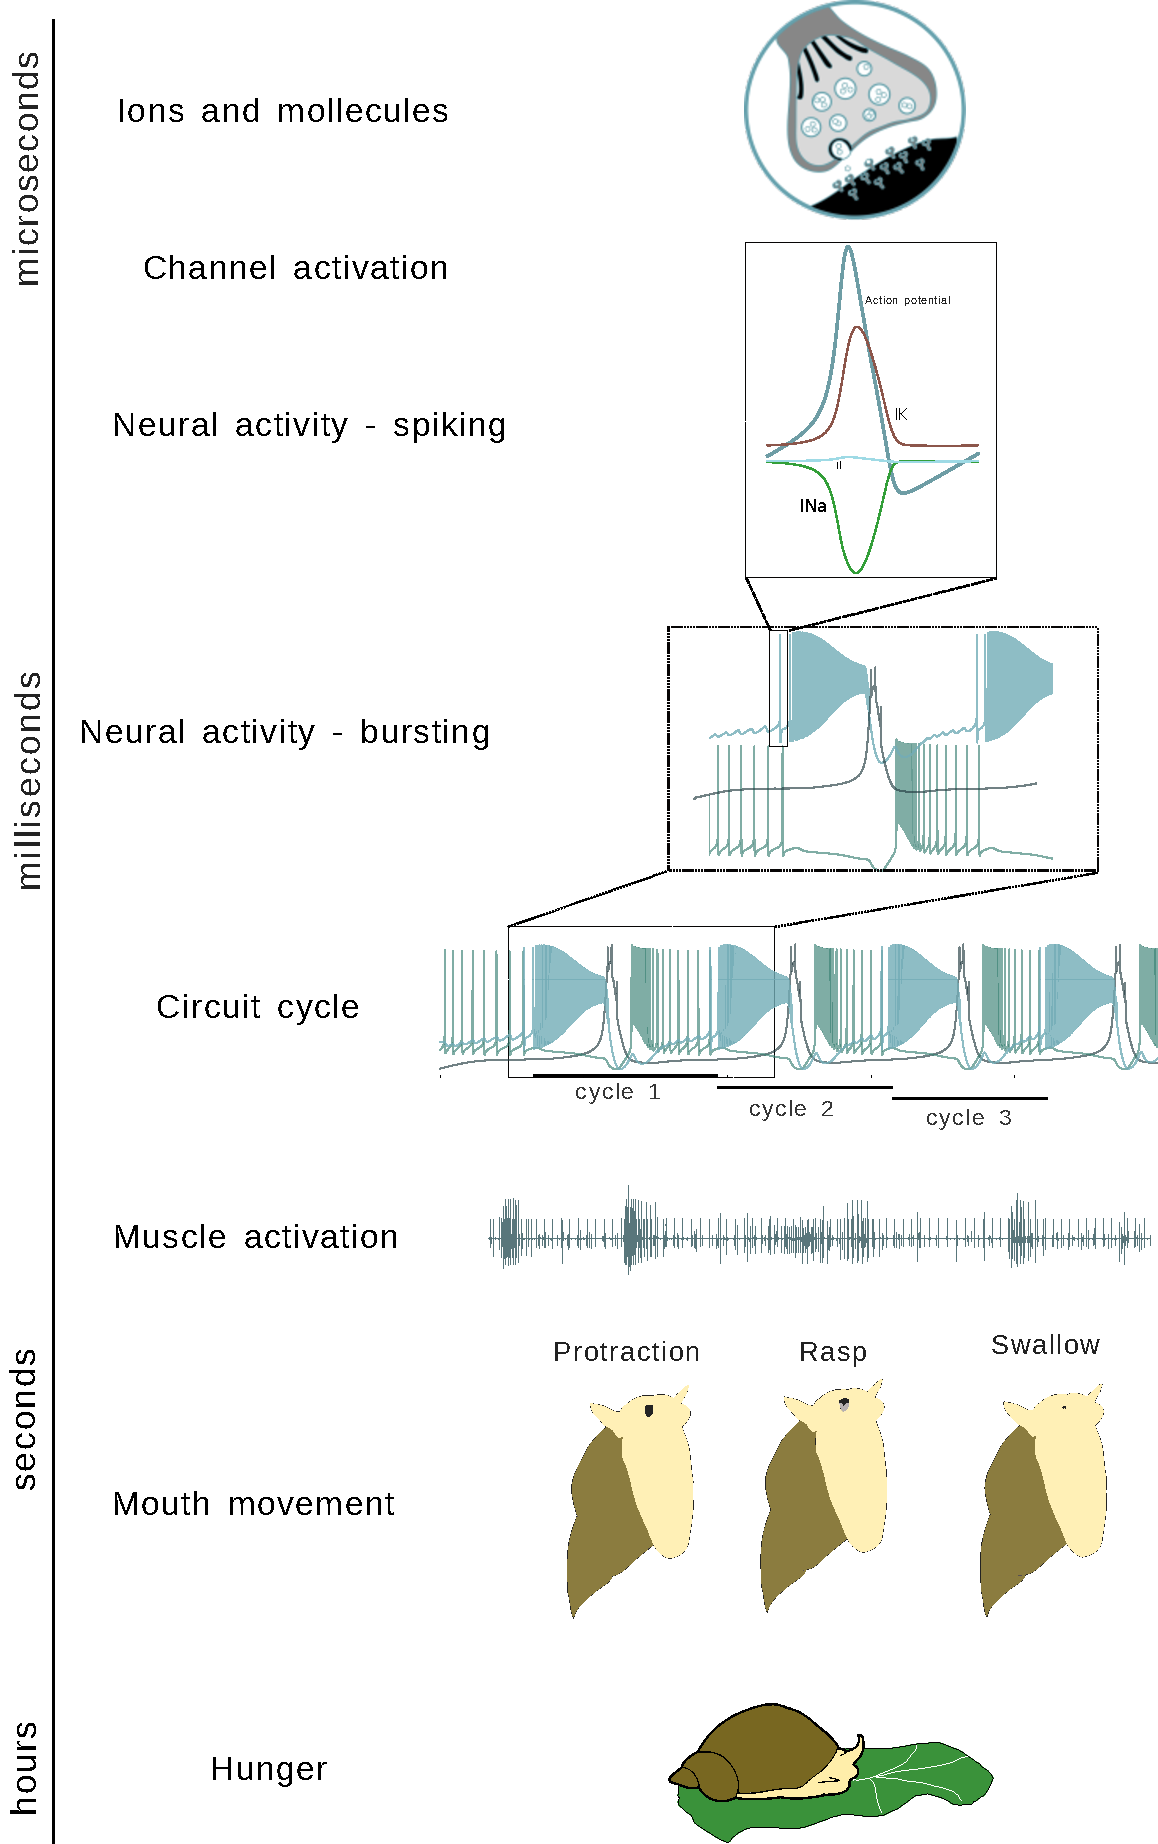
\includegraphics[width=0.9\textwidth]{img/intro/time scale/time-scale-feeding.pdf}
	\caption{Illustration of the sequential feeding process at different time scales.}
	\label{fig:time scale feeding}
\end{figure}

The sequential activity in brain goes from the scale of microsecond to days (see the example of circadian rhythms at \cite{mauk_neural_2004}). In Figure \ref{fig:time scale feeding} there is an illustrative example of the sequential nature of activity at different scales in the generation of coordinated motor activity in the feeding of a snail. At the scale of microseconds, there is a flow of ions that generate a sequence of ionic channel activation, that in the scale of milliseconds produce action potentials. The combination of them in form of rhythmic bursts, activate the corresponding muscles at the scale of seconds and generate the necessary sequential movement to eat: open the mouth, rasp food and swallow, that will be repeated along day. 


Thus, apart from the focus on sensory processing, behavior and cognition (large temporal scales and top-bottom approaches), the study of the action potential dynamic and the interaction between ionic channels and synapses is crucial, since it is a key part in any brain process so it cannot be detached from the whole. The alteration of these channels at different sites along the neuron can affect synaptic inputs/outputs, how the neurons communicate and the resulting process. Ionic channels are the starting point of the electrical signal generated underlying neuronal network activity, and a malfunction of it can contribute to neuronal disorders \parencite{kecskes_editorial_2023}. Thus, understanding brain activity not only at large scales but from the voltage generation dynamics can be crucial for a real and complete brain understanding. Their study can also help distinguish between short- and long-term modulation, a key aspect in neural plasticity and the application of neuromodulatory techniques \parencite{chambers_light-activated_2008,burke_modulation_2019}.

%Regarding sequential studies, it is common to talk about neural activity as blocks of information and as a binary on-off event, even for whole brain areas, classifying tasks by those findings. Although the findings under this approach have been undoubtedly relevant, they usually do not consider the importance of dynamics, variability and how their processing affects behavior.
 
%Although often disregarded in macroscopic studies and as a consequence in bottom-up approaches,
It is important to explore the mechanisms that allow to maintain a robust sequential activity despite changes in context and the variability underlying the neural dynamics. Action potentials and bursts are classified as we have seen depending on their waveform shape and grouped activity, however in those subgroups there is a high intra-variability, where for example bursting activity can differ in shape and duration, i.e., number of spikes in a bursts. In Figure \ref{fig:burst variability} there is an example of the variability in the burst waveform and duration for a sequence of several bursts. 


\begin{figure}[htb!]
	\centering
	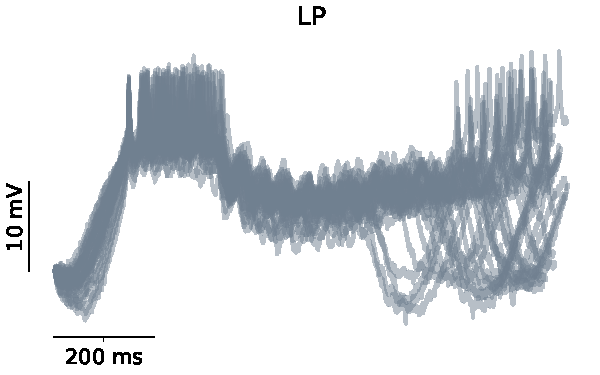
\includegraphics[width=0.6\textwidth]{img/intro/burst_variability.pdf}
	\caption{Superimposition of bursts at different time instants aligned by the first point of the segment for intracellular recordings of an LP neuron in the sthomatogastric CPG.}
	\label{fig:burst variability}
\end{figure}



The study of this variability unveils key factors in the sequentiallity and how it is maintained despite of the alterations in the medium. This is the case for example of dynamical invariants, i.e., strong relationships between time intervals that conform a cycle of activity, when analyzing the activity cycle-by-cycle \parencite{reyes_artificial_2008,elices_robust_2019,garrido-pena_characterization_2021,berbel_emergence_2024}. This dynamical invariants might have a crucial role understanding the robustness of sequential activity and the relation between variability, robustness and flexibility found in many brain processes \parencite{citas}. We will discussed in detail this phenomena in the feeding CPG of \textit{Lymnaea stagnalis} in chapter \ref{c-invariants}.


\section{Studying neural dynamics in computational models.}
\label{sec:computational neuroscience}
Computational Neuroscience is a subfield of neuroscience that enhances the theoretical and computational techniques to address the study of nervous system functioning at multiple levels, from molecular level to complex networks or behavior. It is then by definition, a multi-disciplinary field. The basis of Computational Neuroscience lay on the understanding of brain dynamics from its electrical signals and the information they carry \parencite{schwiening_brief_2012,catterall_hodgkin-huxley_2012,dimitrov_information_2011,shannon_mathematical_1948}. Computational Neuroscience has extended its scope, leading to new paths of research including complex networks, graph theory, single cell analysis and machine learning techniques \parencite{cns2023}. In fields such as Artificial Intelligence there is even a symbiotic relationship between fields, where both inspire and help each other grow \parencite{amunts_human_2019,wozniak_deep_2020,goncalves_training_2020}.

An important part of Computational Neuroscience is the description of living dynamics with theoretical models and the reproduction of their activity by the model simulation. The simulation of neural activity is a powerful tool to explore the neuronal dynamics, biophysical sources and possible mechanisms underlying the neural signaling, behavior, etc. Its strength relies on the reproducibility, extensive range of tunable parameters and the ability to modify (include/exclude) elements in the system or circuit. Although models cannot fully substitute research on living systems, they do lead us closer to the insight of neural dynamic, being a fast, effective and less costly alternative to advances in science. Their strength in reproducing brain processes also relies in the similarity to the brain dynamics and its signal processing. Also, models are an essential complement reaching detailed descriptions where experimental approaches such as electrophysiology have their limitation. 
%Like science is not about truth, but about knowledge, models do not aim to substitute living systems, but to lead us closer to the insight of neural dynamics. %#ToDo revisar

Models can be classified by their level of specification, i.e. what level of abstraction is decided in neural dynamics, the structure being modeled and the size of the network, or their ability to reproduce chaotic activity. In Figure \ref{fig:models-classification} there is a colored box illustrating this classification, with examples of models of large networks as \cite{potjans_cell-type_2014,bezaire_interneuronal_2016}, of single cell but still detailed as in \cite{smith_dendritic_2013} and more abstract descriptions as in \cite{izhikevich_simple_2003}. Regarding the level of description, in the different biophysical models there is always a choice between high description of non-linearities, channels and excitation properties, and efficiency in computation. In this line, from \cite{hodgkin_quantitative_1952} model, rich in the description of nonlinearities, \cite{hindmarsh_model_1984} defined with polynomial equations, similar neuronal dynamics. \cite{fitzhugh_impulses_1961}, defined a model substituting a detailed description of nonlinearities by a fast and slow description of the dynamics (see \cite{torres_modeling_2012} for a review of this models). 


%Adapt models table from
%https://www.sciencedirect.com/science/article/pii/S0896627319304441 Figure 2A:
\begin{figure}[bth!]
	\centering
	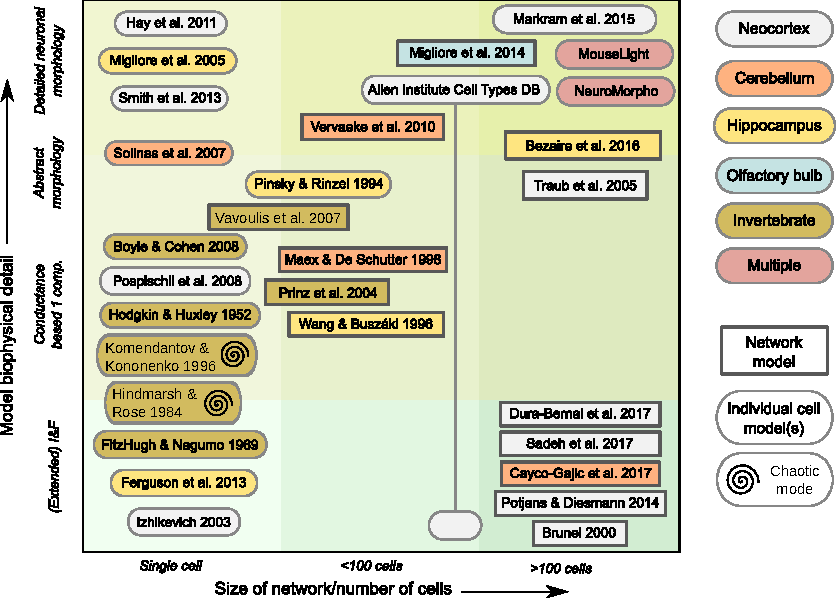
\includegraphics[width=\textwidth]{img/intro/models classification.pdf}
	\caption{Neural and network models classified by biophysical detail, structure modeled and size of the network. Figure adapted from Figure 2 \cite{gleeson_open_2019} under \href{http://creativecommons.org/licenses/by/4.0/}{Creative Commons CC-BY license}. Models are classified by the biophysical detail, by y-axes being the models in the bottom the less specific ones; by the size of the network modeled, from left to right one cell to hundreds of cells; and by the brain-structure they model, represented in colored boxes. The shape of the box also classifies the model in network model or individual cell model. A third category was here included from the original work, representing by an spiral in the box the ability of the model to produce chaotic activity without external alterations, i.e, reproduce spontaneous variability.}
	\label{fig:models-classification}
\end{figure}

\subsection{Conductance-based models}

In this thesis, all experimental recordings have been supported with simulations on conductance-based models. They are defined as mathematical descriptions of the ionic channels dynamics, based on their electrical signal. The pioneer study \cite{hodgkin_quantitative_1952} model defined dynamical equations based on the electrical circuit of neurons in \textit{Aplysia}, similar to the one described in \ref{fig:electrical circuit}. This modeled circuit is also used to conform the intracellular recording configuration, where the pipette is included as an extra current compensated by the electrode in the bath (see Fig. \ref{fig:clamp circuit}).

\begin{figure}[htb!]
	\centering
	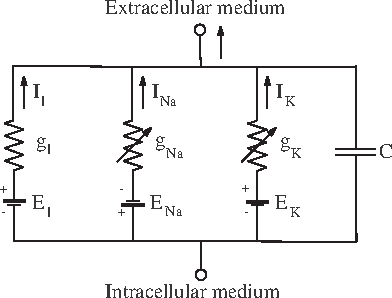
\includegraphics[width=0.7\textwidth]{./img/intro/electrical_circuit.pdf}
	\caption{Electrical circuit describing the membrane voltage model.}
	\label{fig:electrical circuit}
\end{figure}

\begin{figure}[htb!]
	\centering
	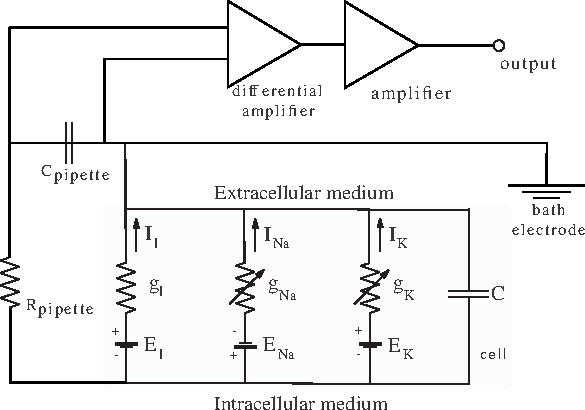
\includegraphics[width=0.7\textwidth]{./img/intro/intracellular_recording_circuit.pdf}
	\caption{Electrical circuit representing the scheme for intracellular recordings.}
	\label{fig:clamp circuit}
\end{figure}


In these models, the simulation of neural electrical activity is based on the mathematical description of different ionic channels in the circuit, whose dynamics are also well defined by activation gates. First, there is a mathematical description of the Voltage dependent on time, as described equation \ref{eq:voltage ions}:

\begin{equation}
 C_m \frac{dV}{dt} = I - \sum I_{x},
  \label{eq:voltage ions}:
\end{equation}

where $I_{x}$ is the current description for each channel involved in the action potential generation, e.g. $I_K$, $I_{Na}$, $I_{Ca}$.

Second, each channel is also described as a differential equation, voltage-dependent composed by activation-gates dynamics:
\begin{equation}
I_x =  g_x \sum act_{vars}^n (V - E_x), 
\end{equation}

where $g_x$ is the corresponding conductance of the channel, $E_x$ is the reversal potential for that channel.
Activation gates usually have an exponential tendency, and are defined by activation and inactivation dynamics, also dependent on voltage and time. They follow the structure in equation \ref{eq:alpha-beta}

\begin{equation}
	\label{eq:alpha-beta}
	\frac{act}{dt} = \frac{act_{\infty,i}-act_i}{\tau_{act,i}}
\end{equation}

where $\tau_{act,i}$ are the relaxation time constants which are usually voltage-dependent and modeled using sigmoid or Gaussian functions. 


Following the \cite{HODGKIN1952} description, an example of the equations corresponding to figure \ref{fig:electrical circuit} are described in the following table:
%\begin{equation}
%		C \frac{dV}{dt} = I - g_K n^4 (V - E_K) - g_{Na} m^3h(V-E_{Na}) - g_L (V-E_L)
%\end{equation}

% Please add the following required packages to your document preamble:
% \usepackage{multirow}
\begin{table}[h!]
	\begin{tabular}{lccc}
		Voltage equation                                                                 & \multicolumn{3}{c}{$C \frac{dV}{dt} = I - g_K n^4 (V - E_K) - g_{Na} m^3h(V-E_{Na}) - g_L (V-E_L)$}                                                                                                                                  \\ \hline
		& \multicolumn{2}{c}{Activation variables}                                                                                                                              & Inactivation variable                                        \\ \hline
		\multicolumn{1}{c|}{\begin{tabular}[c]{@{}c@{}}gating \\ variables\end{tabular}} & \multicolumn{1}{c|}{$\frac{dm(t)}{dt}=\frac{m_{\infty}(V(t))-m(t)}{\tau_m(V(t))}$} & \multicolumn{1}{c|}{$\frac{dn(t)}{dt}=\frac{n_{\infty}(V(t))-n(t)}{\tau_n(V(t))}$} & $\frac{dh(t)}{dt}=\frac{h_{\infty}(V(t))-h(t)}{\tau_h(V(t))}$ \\ \hline
	\end{tabular}
%	\begin{tabular}{cccc}
%		\multicolumn{1}{l}{Voltage equation}                                                              & \multicolumn{3}{c}{$C \frac{dV}{dt} = I - g_K n^4 (V - E_K) - g_{Na} m^3h(V-E_{Na}) - g_L (V-E_L)$}                                                                                                       \\ \hline
%		\multicolumn{1}{l}{}                                                                              & \multicolumn{2}{c}{Activation variables}                                                                                                                 & Inactivation variable                          \\ \hline
%		\multicolumn{1}{c|}{\begin{tabular}[c]{@{}c@{}}gating \\ variables\end{tabular}}                  & \multicolumn{1}{c|}{$n = \alpha_n (V)(1-n)-\beta_n(V)n$}                    & \multicolumn{1}{c|}{$m = \alpha_m (V)(1-m)-\beta_m(V)m$}                   & $h = \alpha_h (V)(1-h)-\beta_h(V)h$            \\ \hline
%		\multicolumn{1}{c|}{\multirow{2}{*}{\begin{tabular}[c]{@{}c@{}}transition \\ rates\end{tabular}}} & \multicolumn{1}{c|}{$\alpha_n(V)=0.01\frac{10-V}{\exp(\frac{10-V}{10})-1}$} & \multicolumn{1}{c|}{$\alpha_m(V)=0.1\frac{25-V}{\exp(\frac{25-V}{10})-1}$} & $\alpha_h(V)=0.07\exp\frac{-V}{20}$            \\ \cline{2-4} 
%		\multicolumn{1}{c|}{}                                                                             & \multicolumn{1}{c|}{$\beta_n(V)=0.0125\exp(\frac{-V}{80})$}                 & \multicolumn{1}{c|}{$\beta_m(V)=4\exp(\frac{-V}{18})$}                     & $\beta_h(V)=\frac{1}{\exp(\frac{30-V}{10})+1}$ \\ \hline
%	\end{tabular}
	\label{table:hh-equations}
\end{table}

That combination of channels generates the spike waveform showed in Fig. \ref{fig:spike-types model}a) but, as in living systems, the combination of different channels lead to distinct outputs, e.g. shoulder and no-shoulder type neurons (see previous section, Fig. \ref{fig:spike-types}). This is the case of waveform in Fig. \ref{fig:spike-types model} b), where this shoulder shape could be reproduced in models by including specific channels, e.g., calcium channels.

\begin{figure}[htb!]
	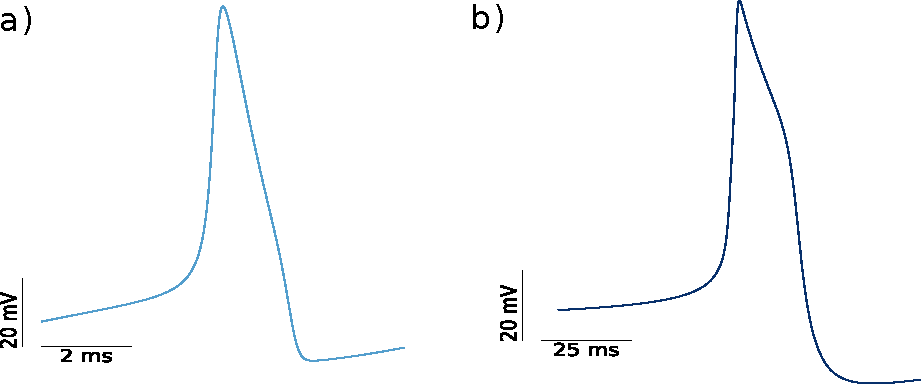
\includegraphics[width=\textwidth]{img/intro/spike-types model.pdf}
	\caption{Simulation of two distinct spike types: no shoulder (a) and shoulder shaped (b), described by equations in \cite{hodgkin_quantitative_1952} and \cite{vavoulis_balanced_2010}, respectively}
	\label{fig:spike-types model}
\end{figure}

\subsubsection{\large{Modeling networks}}
Apart from the modeling of the action potential generation, synapses can also be modeled depending on the type and the level of specificity. Synapses are defined in conductance-based model as an extra current, that simulates the alteration in the neuron dynamics by chemical or electrical synapses. In conductance based models, electrical synapses are usually defined by the following equation:
\begin{equation}
    I_{ij}(t) = \bar{G}_{ij} (V_i(t) - Vj(t))
\end{equation}
\noindent where $i$ and $j$ represent the two neurons conforming the electrical synapse and $\bar{G}_{ij}$ is a constant representing the maximum value of synapse conductance in the connection.

On the other hand, chemical synapses are by definition asymmetrical and can be described as in equation \ref{eq:synapse binary}:
\begin{equation}
     I_{ij}(t) = G_{ij}(t) (V_i - E_j^{syn})
     \label{eq:synapse binary}
\end{equation}
\noindent where $E_j^{syn}$ is the voltage value at which the synaptic current cancels and $G_{ij}$ can now have complex dynamics considering the trafficking of neurotransmitters as in equation \ref{eq: Gii} \parencite{torres_modeling_2012}. 

\begin{equation}
	G{ij}(t) = \bar{G_{ij}}  \Theta(t-t_j^{sp}) \alpha (t-t_j^{sp})
	\label{eq: Gii}
\end{equation}

Depending on the selection of this level of specification, the neuron can be activated by a (i) binary cause: occurrence or absence of an action potential, or (ii) a dynamic model that is also dependent on the voltage variations. In that second case the level of specification is higher, with a richer description of the synapse dynamics. This is the case for example of \cite{tsodyks_neural_1997}, represented in equations \ref{eq:tsodyks1},\ref{eq:tsodyks2} or the gradual synapse in the CPG model by \cite{vavoulis_dynamic_2007}, discussed in methods chapter, section \ref{sec:CPG model}.


\begin{equation}
	\frac{dU}{dt} = -\frac{U}{\tau_{\text{rec}}} + U_{\infty}(1 - U) \delta(t - t_{\text{spike}})
	\label{eq:tsodyks1}
\end{equation}
\begin{equation}
	\frac{dX}{dt} = -\frac{X}{\tau_{\text{fac}}} + (1 - X) \frac{U(t_{\text{spike}})}{U_{\infty}} \delta(t - t_{\text{spike}})
	\label{eq:tsodyks2}
\end{equation}


\subsection{Variability in computational models}

Although it was included in the general model classification in figure \ref{fig:models-classification}, the capability of models to reproduce chaotic activity is often undervalued, as it happens in experimental research. Most studies use deterministic non-chaotic models, which are sufficient when exploring input/output responses, studying the role of different biophysical elements or supporting experimental results. However, living systems are chaotic and highly variable, and still able to produce sequential, constant and reproducible patterned activity. Variability in the activity of living neurons has been proven to play an important role in relevant information processing tasks. While this is a key aspect in neural dynamics, models usually exclude the variability from their description particularly in membrane potential waveforms and in collective adaptive dynamics. To induce stochasticity usually it is included Gaussian noise as external input \parencite{linaro_accurate_2011,pezo_diffusion_2014,zheng_spontaneous_2020}. However, this is limited when exploring the role of variability in the sequences or in the information processing, inferring hypothesis from the model analysis. There are possibilities to include the variability in the own neural dynamics, within its channels, as it is the example of \cite{hindmarsh_model_1984} or \cite{komendantov_deterministic_1996}, where in both descriptions, there is a combination of parameters that lead both to a chaotic state, where the resulting activity is not purely deterministic. When the source of the variability in the system comes from its intrinsic properties there is a possibility to study its dynamics and the role of this variability in the system without artificially induced modifications such as noise in the gaussian or currents, and explore the specific properties of the channels as if it was an spontaneous activity recording.

\todo{añadir cómo consiguen variabilidad?}

\section{Vertebrate and invertebrate animal studies}
\label{c-intro-invertebrates}
Even before computational techniques were an option, the study of Neural dynamics and behavior was carried using many different model animals. Apart from the hegemonic rodents models, there have been invaluable findings using invertebrates as animal models, such as genetics and developmental biology in \textit{C. elegans} \parencite{brenner_genetics_1974}, \textit{Zebra fish} \parencite{streisinger_production_1981} and \textit{Drosophila} \parencite{nusslein-volhard_mutations_1980}; neural dynamics in \textit{Aplysia} \parencite{HODGKIN1952,wachtel_direct_1967}, motor activity in \textit{Carcinus maenas} \parencite{eisen_mechanisms_1982} or \textit{Lymnaea stagnalis} \parencite{Benjamin1979b}, the main animal model in this thesis. Besides those examples, these animal models have been used for a wide variety of fields including behavioral studies, ecotoxicology, evolution, human disease modeling... \parencite{romanova_animal_2018} 

Despite the differences between invertebrates, mammals and concretely human brain, there are many characteristics of animals' systems that can be extrapolated to humans. We should keep in mind that any model animal is still a model, with differences from the real focus of study --the human brain-- and as a model, there are differences in the structure, even in mammal species \parencite{preuss_taking_2000}. So by using computational models or exploring more animal species there can be set a better ground truth for the aspects that shape the neuronal and behavioral dynamics. 

 % https://karger.com/bbe/article-abstract/55/6/287/46613/Taking-the-Measure-of-Diversity-Comparative?redirectedFrom=fulltext  
 %First, by examining a wider range of species than are currently employed, and by using modern techniques of phyletic analysis, neuroscientists can more rigorously identify those features of cortical organization that are, in fact, widely shared among mammals or among particular mammalian subgroups. Second, by taking account of variations, neuroscientists can abstract more reliable and general principles of structure-function relationships in the nervous system. Finally, freed from the doctrine of basic uniformity, neuroscientists can pursue the study of human cortical specializations, and so advance our understanding of what distinguishes humans as a biological species.

Findings in invertebrates are sometimes overlooked, arguing that features in invertebrates cannot be extrapolated to humans. Thus, there are often used mammals by their biological similarity. However, models in invertebrates have proven their utility not only in basic science. We can find examples of this in human diseases, memory, motor activity and neuromodulation. Particularly, in the study of neural processes, the ease of accessibility and finite number of large neurons in the system, have made invertebrates an interesting case of study. In Figure \ref{fig:invertebrates timeline} there is a timeline containing crucial discoveries in Neuroscience, some of them Nobel Prize winners in the last century, as well as current relevant discoveries in the field. 
% https://docs.google.com/spreadsheets/d/16rOG5LSuFMQGHAakeYqcdG26NIZnY4NWtr6TZku_UKs/edit#gid=0

Among the advantages in using invertebrates there are the easy access to the nervous system, the ease of breeding and reproduction or the simplicity of their biological features, that makes possible a full description of it, i.e. the genomic description of \textit{C. elegans} or the nervous system in \textit{Lymnaea stagnalis}. Also some selected species were a main field of study in the last decades, so there is plenty of literature for each one even in different fields. Furthermore, despite the simplicity of these systems, their nervous system is still capable of generating robust sequential neural activity, preset behavior and even learning processes. 


Apart from the possible advances in science from a productivist view, invertebrates models can also bridge the gap between resources and science, allowing low-income labs and countries to \textit{do} science. This animal models are usually cheaper to obtain, maintain and there is usually a possibility of breeding own colonies. This makes their use extendable and breaks some economical barriers in science, where high-income countries usually centralize the science production with strong conventions \parencite{castillo_spineless_2017,stephan_how_2015}. 

%\textit{What can computational neuroscience provide to experimental approaches}

However, in any animal model is still good to remember that the aim in science and progress should be advances in science but not at all costs. Alternatives such as computational models should be a predefined complement to experimental studies, reducing their necessity and leading to a less harmful alternative to the human's necessity of knowledge. \todo{revisar si quitar}


\subsubsection{\textit{Lymnaea stagnalis}, the great pond snail}
Besides the potential of research in invertebrates in general, here we explore neural system in the great pond snail, \textit{Lymanea stagnalis}. This mollusk has been an important case of study since the late XX century, when it was used extensively to study neurobiological processes and nervous system functioning. This carreer-time effort lead to a detailed description of the buccal ganglia 
%\begin{wrapfigure}{l}{0.3\textwidth}
%	\centering
%	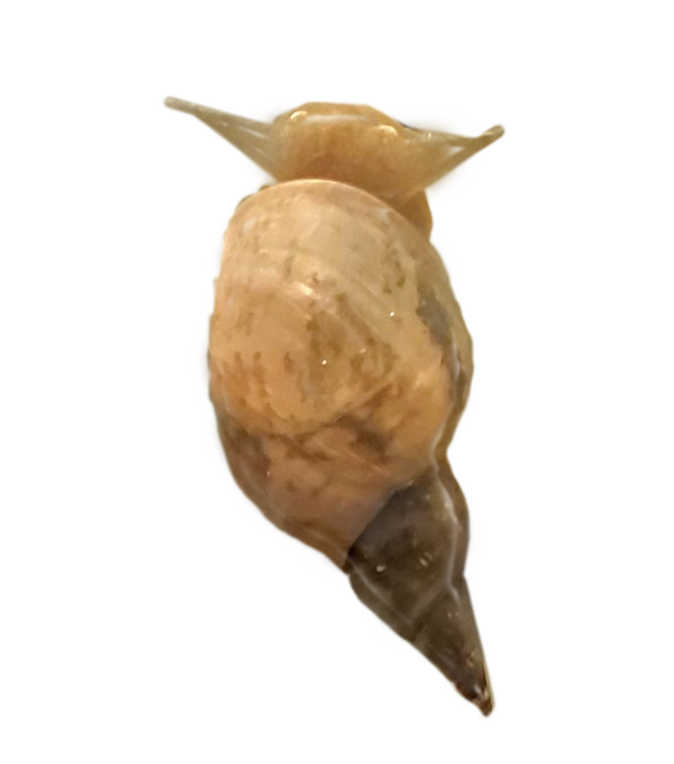
\includegraphics[width=0.7\linewidth]{img/intro/lymnaea.png} 
%	\caption{\textit{Lymnaea Stagnalis}}
%%	\label{fig:snail}
%\end{wrapfigure} 
in its CPG, including the three main interneurons conforming it \parencite{benjamin_snail_1989,benjamin_morphology_1979,rose_relationship_1979,brierley_behavioral_1997}, the modulatory neurons that influence the CPG activity such as SO and CGC neuron in the cerebral ganglia \parencite{rose_interneuronal_1981,mccrohan_patterns_1980,kemenes_multiple_2001}). Besides the buccal ganglia, it is also well identified neurons in other ganglia, with specific characteristics such as electrical coupling or dopamine containing neurons as in Parietal Ganglia \parencite{benjamin_electrotonic_1986,winlow_multiple_1981})

\begin{figure}[htb!]
	\begin{minipage}{0.35\textwidth}
	\centering
	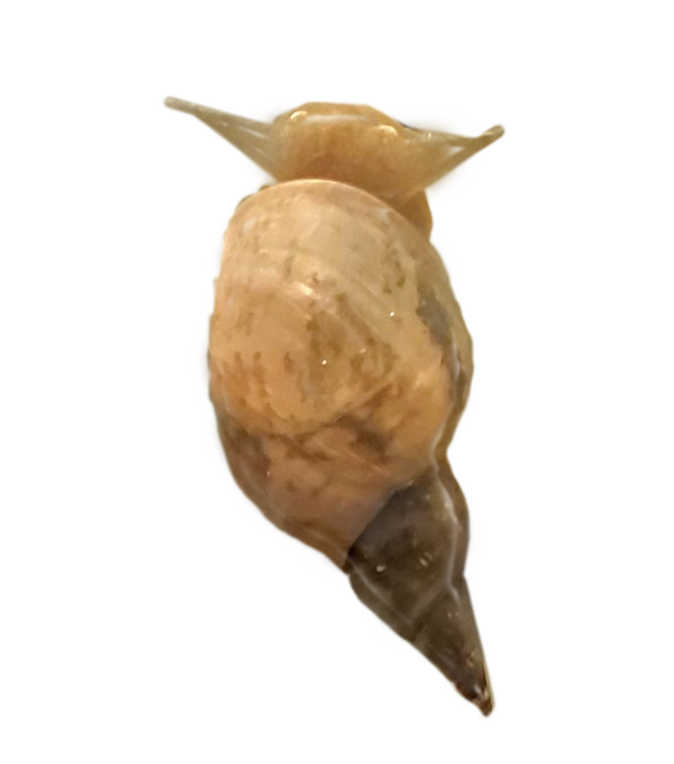
\includegraphics[width=\linewidth]{img/intro/lymnaea.png} 
	\caption{Imagen of \textit{Lymnaea Stagnalis}}
	\label{fig:snail}
	\end{minipage}
	\hfill
	\begin{minipage}{0.65\textwidth}
		\centering
		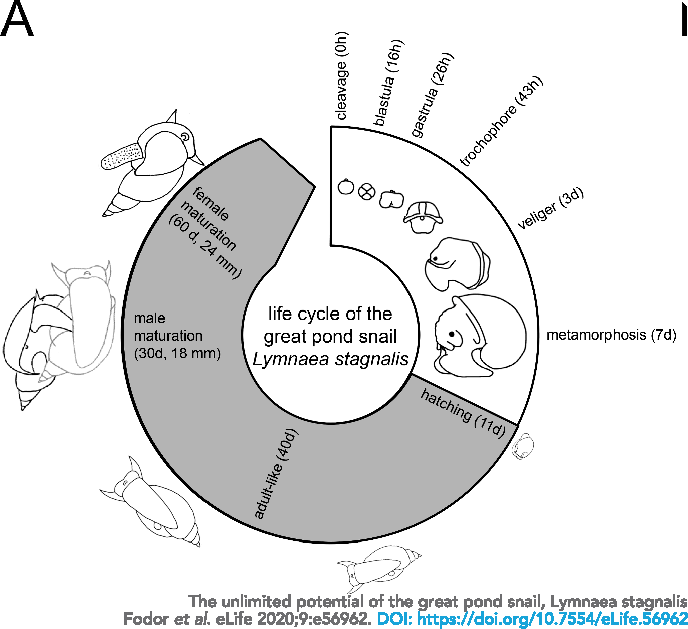
\includegraphics[width=\textwidth]{img/intro/lymnaea_life_cycle.pdf}
		\caption{Representation of \textit{L. stagnalis} life cycle. Figure 2A from \cite{fodor_unlimited_2020} (\href{http://creativecommons.org/licenses/by/4.0/}{Creative Commons license}).}
		\label{fig:lymnaea_life_cycle}
	\end{minipage}
\end{figure}

 From that point on it has been key in other fields as host-parasite or genome editing. This last field is thanks to the short and well studied life-cycle in \textit{L. stagnalis} (see Figure \ref{fig:lymnaea_life_cycle}), as well as the easiness to lab-bread them, without losing its main characteristics through generations \parencite{noland_observations_1946}. Recordings and analyses in this work are framed in the study of neural activity in it central nervous system (CNS). \textit{L. stagnalis} CNS is composed by 11 ganglia that conform the system: symmetrical pairs of buccal, pedal, cerebral, pleural and parietal, and a single visceral ganglia (see Sec. \ref{sec:lymnaea morphology}). We will focus specially in its feeding CPG, that by a distributed combination of motor- and inter-neurons allocated mainly in buccal and cerebral ganglia, produce a rhythmic pattern movement that allows feeding in three phases (protraction, rasp and swallow). Apart from this study of the CPG we will work on the giant neurons located in the right parietal ganglia (RPG), enhancing the high-voltage (up to 80mV) and slow activity (30 to 100 ms per spike) to analyze in detail the action potential dynamics. 


\section{Neural stimulation}
\subsection{Stimulation techniques}

Neural stimulation have been an essential aspect in the study of neural dynamics, allowing the alteration of the neural system to explore, reproduce and alter its dynamics for their study. There are several techniques to produce the stimulation, we could classify them in chemical --using chemical components to block/enhance neural mechanisms--, electrical --injecting current in the cell membrane or nerves-- or optical --where neurons or circuits are stimulated though a illumination process. In this thesis we are going to focus in the last two. In the electrical techniques, since the firsts applications of electrophysiology by \cite{neher_single-channel_1976} and the subsequent apparition of patch-clamp technique \cite{hamill_improved_1981}, many different techniques have been developed, for distinct systems. Voltage-clamp and patch clamping modified the paradigm in physiology and basic medicine in the study of the cell membrane dynamics with an exceptional detail that still today is heading ranges of precise recording and stimulation \parencite{hamill_improved_1981}. To Voltage-clamp followed variations such as dynamic-clamp, that enhances the electrophysiology possibilities by combining it with the possibilities of computing through a closed-loop protocol in real-time \parencite{nowotny_dynamic_2022}. This allows implementing specific algorithms to intervene the neural activity and test it to different approaches \parencite{chamorro_generalization_2012}. 
Regarding optical stimulation, a novel and widespread technique is opto-genetics, that by genetically modifying the animals, neurons are reactive to light and have had great achivements in the last decades using for both stimulation and exploration \parencite{chen_roles_2022}. Other example still understudy is near-infrared laser, a novel technique that will be explored in detail along this thesis. This technique have proven its potential for neuronal stimulation in different systems such as the hippocampus \parencite{liang_temperature-dependent_2009}, spinal ganglia in the cochlea \cite{goyal_acute_2012, barrett_pulsed_2018, brown_thermal_2020} and other systems \parencite{shapiro_infrared_2012, cayce_infrared_2014, begeng_activity_2022}.

%
%Apart from their possible subsequent aplication in clinical application, the use of these techniques for basis science is essential for a clear understanding of their implications, the biophysical mechanism they are able to alter and its safety range, and also for a wide understanding of the brain functioning.

\subsection{Neuromodulation and its need for clinical applications}


Beyond the necessity for neural stimulation in basic research to understand and explore the brain signaling and dynamics, there is a direct social impact for neural stimulation in clinical applications. In this context, Neuromodulation is an area of medicine involving many specialities that can be defined as "the science of how electrical, chemical and mechanical interventions can modulate distinct models of the nervous system function [and it is] inherently non-destructive, reversible, and adjustable" \parencite{krames_neuromodulation_2009}. This field is so important due to its possibilities in brain disorder treatments, for functional stimulation but also by the long-term modulation through neuronal plasticity. Neuromodulation area can be classified, depending on the technology used for it, as invasive or non-invasive. Invasive technologies are those that require a direct interaction with the living system or even a surgery for its modification. A well-known example of this type is deep-brain stimulation (DBS), this technique has been effectively used to treat movement disorders by electrically stimulating the brain at certain brain areas after implanting a device by surgery \parencite{limousin_long-term_2019, hariz_deep_2022}. In the case of non-invasive neuromodulation we can find transcranial magnetic stimulation (TCM), that by electric fields stimulates certain areas of the brain, successful for example in the treatment of depression or obsessive compulsive disorder \parencite{valero-cabre_transcranial_2017, clarke_patients_2018}. Each type of technique has its own advantages, invasive techniques are usually more precise in space and time, whereas non-invasive techniques provide more flexibility and adaptability to different patients and the spreadness of the technique. In this context, the optical techiniques discussed for stimulation in basic research, have been rising in popularity also for clinical applications. 











